\documentclass{beamer}
%%%%%%%%%%%%%%%%%%%%%%
% basic tutorial in german: http://www2.informatik.hu-berlin.de/~mischulz/beamer.html
%%%%%%%%%%%%%%%%%%%%%%

%------- packages ---------%
\usepackage[english]{babel}         %Umlaute, neue deutsche Rechtschreibung
\usepackage[utf8x]{inputenc}        %Kodierung festlegen, für UTF-8 Unterstützung entsprechend 
\usepackage{amsmath,amsfonts,amssymb}   %math. Symbole und Umgebungen
\usepackage{graphicx}
%\usepackage{natbib}

%------- theme and style ---------%
\usetheme{Boadilla}  %% Themenwahl
\usecolortheme{default}
\usefonttheme{default}
\useinnertheme{circles}     %	{circles | default | inmargin |	rectangles | rounded}
\useoutertheme{default} %	default | infolines | miniframes | shadow | sidebar | smoothbars |smoothtree | split | tree}
%\beamertemplatenavigationsymbolsempty   % disable navigation simbols
%\bibliographystyle{apalike}
%------- metainformation ---------%

\title[Bifurcation]{Bifurcation in parameter dependent systems\\~\\}
\subtitle{Numerical Methods for Systems Biology WS 12/13}
\author[Jonas Ibn-Salem]{Jonas Ibn-Salem}
\institute[]{}
\date{10.01.13}
%\logo{\pgfimage[width=2cm,height=0.5cm]{grafik/FULogo_RGB}}
\titlegraphic{
\includegraphics[width=4cm,height=1cm]{grafik/FULogo_RGB}}


\begin{document}
%\frame{\titlepage}
\maketitle


\begin{frame}{Overview}
    \tableofcontents
\end{frame}

%%%%%%%%%%%%%%%%%%%%%%%%%%%%%%%%%%%%%%%%%%%%%%%%%%%%%%%%%%%%%%%%%%%%%%%% 
\section{Introduction: Fixed Point Analysis}
%%%%%%%%%%%%%%%%%%%%%%%%%%%%%%%%%%%%%%%%%%%%%%%%%%%%%%%%%%%%%%%%%%%%%%%% 
\begin{frame}{Introduction: Fixed Point Analysis}
    Given the system of differential equations:
    $$y' = f(y) $$
    \begin{definition}
        A \emph{fixed point $y^*$} is defined by $f(y^*)=0$.
    \end{definition}
    %$\Rightarrow$ 
    \begin{itemize}
        \item Solve the equation $f(y) = 0$ 
        \item Analyse eigenvalues of the Jacobian at fixed points.
    \end{itemize}
    Now: System with \emph{controle parameter} $\mu$. 
    $$y' = f(y, \mu)$${}    
    $\Rightarrow$ How does $\mu$ influence the number, location and stability of fixed points?
\end{frame}
%%%%%%%%%%%%%%%%%%%%%%%%%%%%%%%%%%%%%%%%%%%%%%%%%%%%%%%%%%%%%%%%%%%%%%%% 
\section{Bifurcation}
%%%%%%%%%%%%%%%%%%%%%%%%%%%%%%%%%%%%%%%%%%%%%%%%%%%%%%%%%%%%%%%%%%%%%%%% 

\begin{frame}{Bifurcation}
    \begin{definition}
        \emph{Bifurcation} is the changing of the character of an equalibrium point and/or the creation of extra ones by alteration of a control parameter.
    \end{definition}

\end{frame}

\subsection{Example: Logistig growth with harvesting}
\begin{frame}{Example: Logistig growth with harvesting}
    Growth of a population:
    $$y' = \frac{1}{10}y(10 - y) - \mu $$

    Solving $f(y,\mu) = 0$ for any parameter $\mu$. 
    %E.g. for $\mu = 0$ fixed points at $y=0$ and $y=10$.
    %For any parameter $\mu$: $\frac{1}{10}y(10 - y) - \mu = 0$
     \begin{columns}
        \column{.25\textwidth}
            Bifurcation Diagram:
        \column{.75\textwidth}
            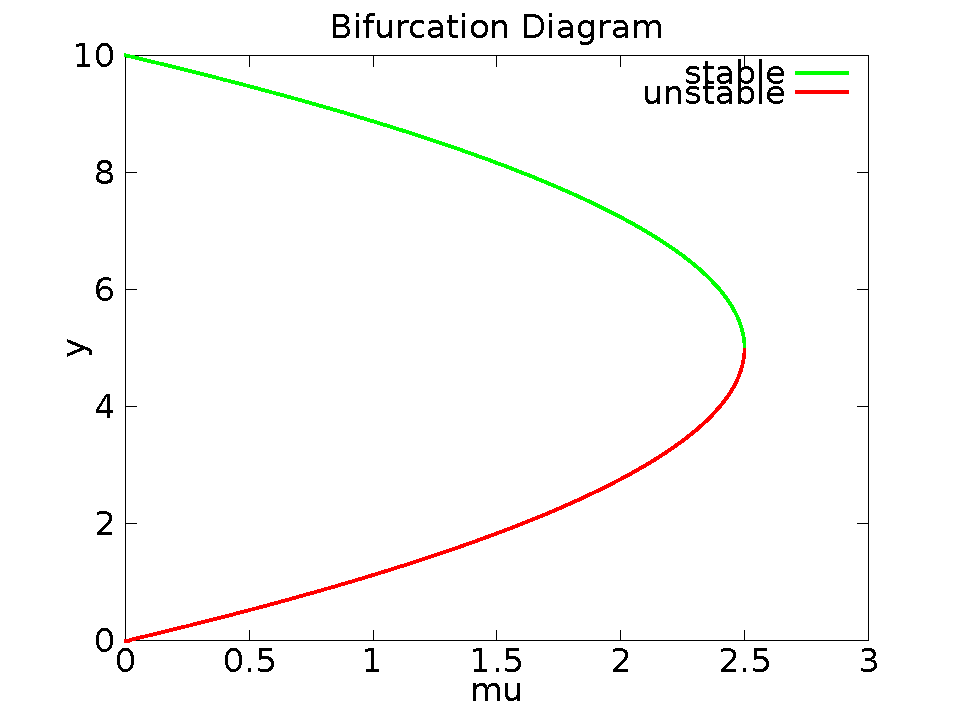
\includegraphics[width=.8\textwidth]{grafik/harvesting}
    \end{columns}
\end{frame}

%%%%%%%%%%%%%%%%%%%%%%%%%%%%%%%%%%%%%%%%%%%%%%%%%%%%%%%%%%%%%%%%%%%%%%%% 
\section{Hopf-Bifurcation}
%%%%%%%%%%%%%%%%%%%%%%%%%%%%%%%%%%%%%%%%%%%%%%%%%%%%%%%%%%%%%%%%%%%%%%%% 


%%%%%%%%%%%%%%%%%%%%%%%%%%%%%%%%%%%%%%%%%%%%%%%%%%%%%%%%%%%%%%%%%%%%%%%% 
\section{Numerical Bifurcation Analysis}
%%%%%%%%%%%%%%%%%%%%%%%%%%%%%%%%%%%%%%%%%%%%%%%%%%%%%%%%%%%%%%%%%%%%%%%% 


\end{document}

